% U-Chrom manuscript — journal-neutral draft.
% Build: latexmk -xelatex main.tex   (or: make)
\documentclass[11pt]{article}

\usepackage{fontspec}
\setmainfont{texgyretermes}[Extension=.otf,UprightFont=*-regular,BoldFont=*-bold,ItalicFont=*-italic,BoldItalicFont=*-bolditalic]  % Times-like body
\setsansfont{texgyreheros}[Extension=.otf,UprightFont=*-regular,BoldFont=*-bold,ItalicFont=*-italic,BoldItalicFont=*-bolditalic]  % Helvetica/Arial-like
\usepackage[a4paper,margin=2.5cm]{geometry}
\usepackage{setspace}
\usepackage[running]{lineno}
\usepackage{graphicx}
\usepackage{authblk}
\usepackage[numbers,sort&compress]{natbib}
\usepackage[labelfont=bf,labelsep=space,font=small,singlelinecheck=false]{caption}
\usepackage{xcolor}
\usepackage[colorlinks=true,linkcolor=blue!50!black,citecolor=blue!50!black,urlcolor=blue!50!black]{hyperref}

\graphicspath{{figures/}}
\newcommand{\todo}[1]{\textcolor{red}{[TODO: #1]}}
\newcommand{\pkg}[1]{\texttt{#1}}

\title{U-Chrom: a unified framework for sequencing- and imaging-based 3-D genome data}
\author[1]{Author One}
\author[1]{Author Two}
\affil[1]{\todo{affiliation}}
\date{}

\begin{document}
\maketitle
\doublespacing
\linenumbers

\begin{abstract}
\noindent\todo{Abstract (background, results, conclusions; $\leq$ 350 words).}
\end{abstract}

\noindent\textbf{Keywords:} 3-D genome, chromatin tracing, Hi-C, single-cell multi-omics, data model, software

\section*{Background}
\todo{Motivation: each assay captures one facet of 3-D genome organisation (Fig.~\ref{fig:overview}a); no shared data model links them.}

\section*{Results}

\subsection*{A shared index for sequencing- and imaging-based 3-D genome data}
\todo{ChromData design (Fig.~\ref{fig:overview}b): modality layers, genomic bins, observation levels, bridges.}

\begin{figure}[p]
  \centering
  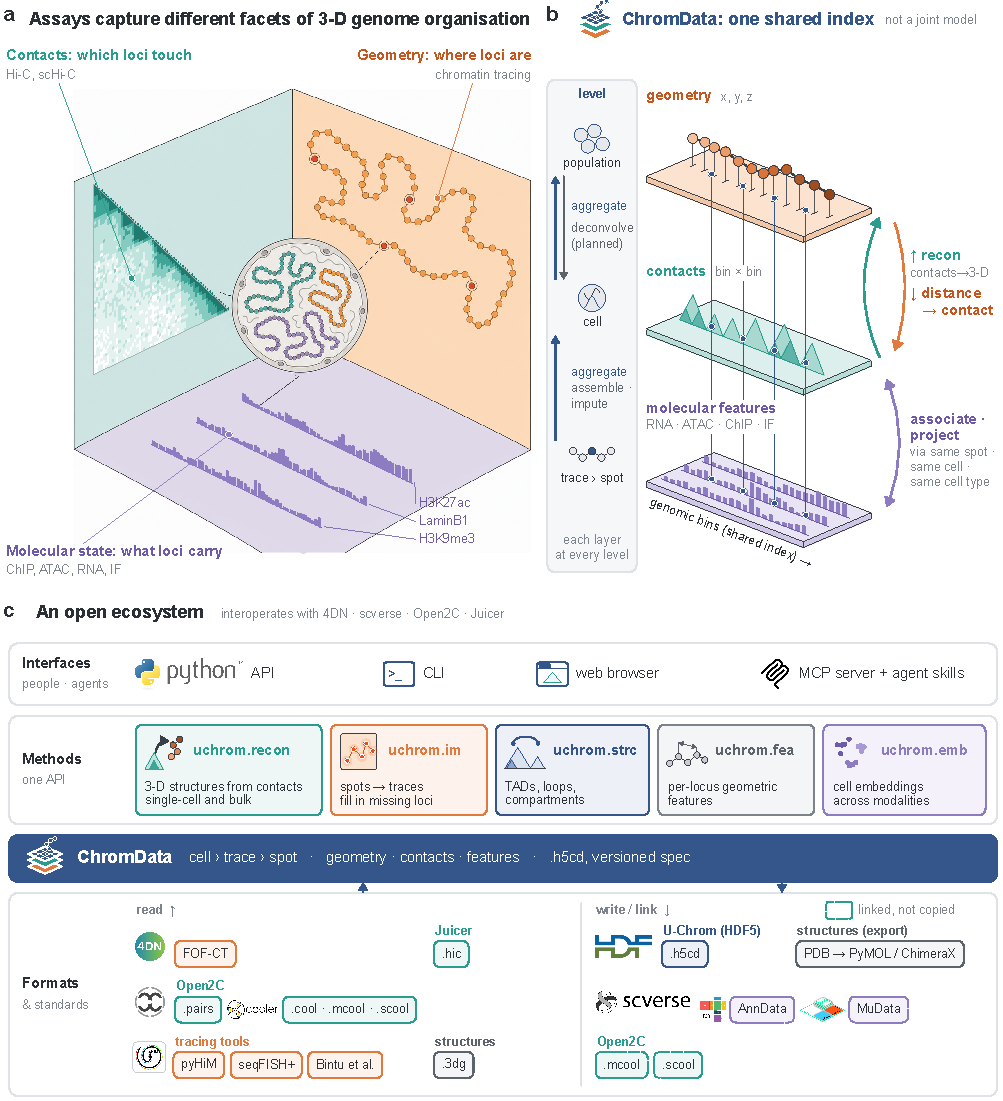
\includegraphics[width=\textwidth]{fig1.pdf}
  \caption[U-Chrom overview]{\textbf{U-Chrom places sequencing- and imaging-based 3-D genome data on one shared index.}
\textbf{a}~Each assay captures a different facet of 3-D genome organisation.
Hi-C and scHi-C measure contacts, that is, which loci touch.
Chromatin tracing measures geometry, where loci are.
ChIP, ATAC, RNA and immunofluorescence (IF) measure molecular state, what loci carry.
The left wall shows the scHiCAR contact map of mouse primary motor cortex (all 5,313 cells merged; chr7:53--68\,Mb; 250-kb bins; ICE-balanced)~\citep{schicar}.
The floor shows H3K27ac, LaminB1 and H3K9me3 IF signals along chr15 in one cerebellar cell (DNA seqFISH+; 48 bins)~\citep{takei2025}.
\textbf{b}~ChromData is a shared index, not a joint model.
Each modality is stored as its own layer: geometry ($x$, $y$, $z$ coordinates), contacts (bin~$\times$~bin maps; large maps are linked rather than copied) and molecular features (RNA, ATAC, ChIP, IF).
The same genomic bins index every layer (dashed lines).
Observation level is independent of modality (left): any layer can be held at the population, cell or trace\,›\,spot level.
Aggregation moves data up a level; spots are assembled into traces and missing loci are imputed; deconvolution from population to cell is planned.
Bridges connect the layers (right): structures are reconstructed from contacts (recon), and distances are converted into contact frequencies.
Molecular features are associated with, or projected onto, the structure layers through a shared spot, cell or cell type.
Plate contents are schematic but derived from the data in \textbf{a}: the smoothed chr15 trace, its IF signals, and TADs from the chr7 window.
\textbf{c}~The U-Chrom ecosystem.
Community formats are read, or linked without copying (dashed boxes).
ChromData is stored as versioned HDF5 (.h5cd), and structures are exported as PDB.
Five analysis modules share one API: reconstruction (\pkg{uchrom.recon}), imaging-side processing (\pkg{uchrom.im}), structure calling (\pkg{uchrom.strc}), geometric features (\pkg{uchrom.fea}) and cell embeddings (\pkg{uchrom.emb}).
The data are accessible through a Python API, a command-line interface, a web browser, and a Model Context Protocol (MCP) server with agent skills.
The illustration in \textbf{a} is AI-generated and edited by the authors; apart from the contact map and signal tracks, it is conceptual.
Logos are trademarks of their respective owners, used for identification only.
\unskip}
  \label{fig:overview}
\end{figure}

\subsection*{One store at real scale, next to the community formats}
\todo{Storage layout, what each format can represent, storage and access by level, analysis beyond RAM (Fig.~\ref{fig:store}); round trips and access by format (Supplementary Fig.~S1), cross-modal groups (Supplementary Fig.~S2), linked vs copied contacts (Supplementary Fig.~S3).}

\begin{figure}[p]
  \centering
  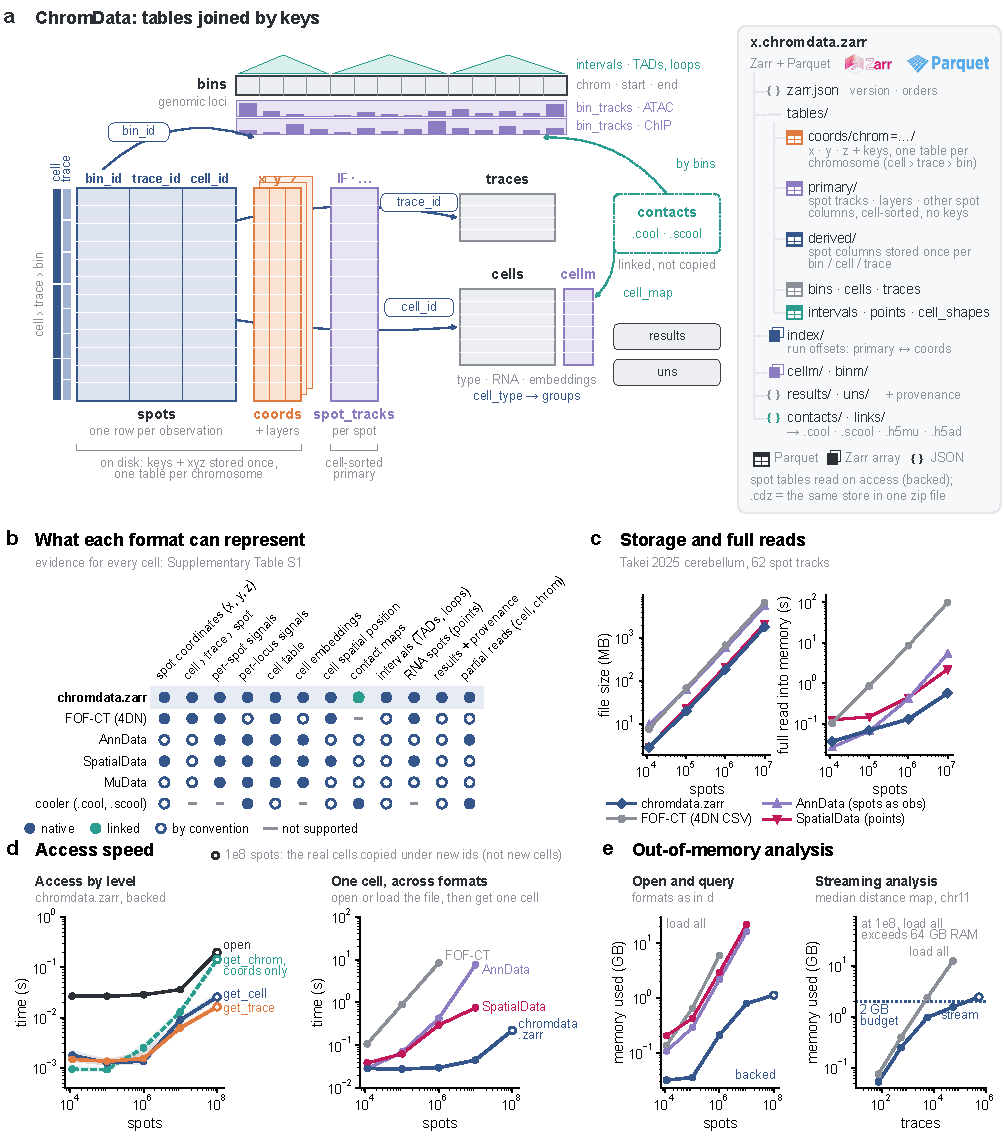
\includegraphics[width=\textwidth,height=0.5\textheight,keepaspectratio]{fig2.pdf}
  \captionsetup{font=scriptsize}
  \caption[ChromData at real scale]{\textbf{One ChromData store serves tracing data at real scale, alongside the formats the community uses.}
\textbf{a}~The ChromData data model: \pkg{spots} (one row per observation) point at a shared locus axis (\pkg{bins}) through \pkg{bin\_id}, and at \pkg{traces} and \pkg{cells} through \pkg{trace\_id} and \pkg{cell\_id}; coordinates (+ layers) and per-spot tracks are row-aligned with the spots, and contact maps are linked by bins and a cell map rather than copied.
Right: the \pkg{x.chromdata.zarr} layout (format 2.2) as written by \pkg{uchrom.core.zarrcd}; the glyph at each node gives its storage type (Parquet table, Zarr array, JSON attributes).
Every spot-aligned value is stored once: coordinates and keys in one Parquet table per chromosome, every other spot-aligned column in cell-sorted primary tables, and spot columns that only repeat a value of their bin, cell or trace once per key; \pkg{index/} maps the (cell, trace, chromosome) runs of the two sides one to one.
\textbf{b}~Interoperability with community formats: what survives an export followed by an import (values compared exactly, coordinates to the format's precision). Filled, preserved; half-filled, partial, or not representable in that format; open, not applicable. PDB is export-only and .3dg import-only in U-Chrom.
\textbf{c}~File size and full-read time (into memory) vs number of spots for whole-cell subsets of the Takei et al.\ 2025 cerebellum DNA seqFISH+ data (62 per-spot tracks)~\citep{takei2025}, for chromdata.zarr 2.2 and the storage schemes publicly used by the community for chromatin-tracing data: the 4DN FOF-CT core table (CSV), AnnData with spots as observations, and SpatialData (spots as a 3-D points element, cells as a table; \pkg{spatialdata} 0.7.2 defaults, full read = \pkg{read\_zarr} + \pkg{.compute()}); median of 3 fresh processes.
At $10^7$ spots chromdata.zarr stores 1.8\,GB and reads in 0.57\,s (FOF-CT 6.7\,GB, 99\,s; AnnData 5.6\,GB, 5.4\,s; SpatialData 2.2\,GB, 2.2\,s).
Flat Parquet, the storage engine under chromdata.zarr and therefore its lower bound without hierarchy, index or metadata, and the ChromData format versions are in Supplementary Fig.~S1.
\textbf{d}~Time per query vs spots: backed chromdata.zarr from disk (\pkg{get\_trace}, \pkg{get\_cell}, \pkg{get\_chrom} with all 62 tracks and with coordinates only, and opening the store; median of 20 random ids $\times$ 3 fresh processes, shading IQR) vs loading the whole table in memory, then subsetting (FOF-CT, AnnData; load + one \pkg{get\_trace}) and SpatialData's lazy route (open + a dask filter on \pkg{trace\_id} + \pkg{.compute()}).
At $10^7$ spots \pkg{get\_trace} takes 6.2\,ms and \pkg{get\_cell} 9.0\,ms; \pkg{get\_chrom} with all tracks reads a slice of every cell-sorted row group (0.52\,s; 13\,ms with coordinates only).
\textbf{e}~Beyond RAM. Left: memory used to open the data and answer the trace and cell queries of \textbf{d} (above the interpreter's baseline), backed chromdata.zarr vs the whole table loaded (colours as in \textbf{d}).
Right: exact median 3-D distance map of chr11, peak memory vs traces when the store is loaded whole and when \pkg{iter\_traces} streams it under a 2\,GB budget (1.55 vs 12.3\,GB at $10^7$ spots); streamed and in-memory medians are bitwise identical at every size (inset: $10^7$ spots, 10.7\,M bin pairs; at $10^8$ against the chromosome loaded alone).
Open markers ($10^8$ spots in \textbf{d} and \textbf{e}): the Takei data replicated ten times with renamed cells and traces, not new cells; at $10^8$ loading the whole table does not fit in 64\,GB of RAM.
\textbf{f}~Groups from one modality, structure from another (scHiCAR mouse primary motor cortex, 5,313 cells)~\citep{schicar}.
Leiden clustering computed in ChromData on the RNA PCA (16 clusters; not the published labels) groups the cells; three contrasting clusters are shown on the RNA UMAP: oligodendrocytes (\textit{Plp1}, \textit{St18}, \textit{Prr5l}, \textit{Mobp}; $n=294$), astrocytes (\textit{Gpc5}, \textit{Slc1a3}, \textit{Atp1a2}; $n=448$) and neurons (no glial or vascular marker expression; $n=1{,}336$).
Their pseudo-bulk contact maps are summed from the linked per-cell .scool through the shared index (the path the web browser uses; chr2:40--90\,Mb, 1\,Mb bins, each normalised to its cis contacts).
Contact probability vs distance, $P(s)$, over all chromosomes: slopes over 2--30\,Mb of $-0.83$ (neurons), $-0.67$ (oligodendrocytes) and $-0.67$ (astrocytes), a modest difference.
Pseudo-bulk from the per-cell .scool equals the published per-type .cool for 22/22 cell types (max $|\Delta| = 0$ over 4.2\,M pixels, all chromosomes).
Right: time to sum the pseudo-bulk of chr1 vs cells aggregated, first query and cached.
Machine: Apple M5 Pro (18 cores), 64\,GB RAM; warm OS page cache.
Zarr and the Zarr logo are marks of the Zarr project (NumFOCUS); Apache Parquet and the Parquet logo are trademarks of The Apache Software Foundation; all logos are used for identification only and do not imply endorsement.
\unskip}
  \label{fig:store}
\end{figure}

\subsection*{An open ecosystem}
\todo{Formats, methods and interfaces (Fig.~\ref{fig:overview}c).}

\section*{Discussion}
\todo{}

\section*{Conclusions}
\todo{}

\section*{Methods}
\subsection*{Data}
\todo{Takei et al.\ 2025 cerebellum DNA seqFISH+; scHiCAR mouse MOp (GSE305439); see \texttt{example-data/README.md}.}

\subsection*{Benchmarks}
Baselines were chosen as the storage schemes publicly used by the community for chromatin-tracing data: the 4DN FOF-CT core table (CSV), AnnData with spots as observations and SpatialData (spots as a 3-D points element), each written and read with its library's defaults.
Flat Parquet, the storage engine under \pkg{chromdata.zarr}, is reported separately as the lower bound without hierarchy, index or metadata (Supplementary Fig.~S1).
The capability comparison (Fig.~\ref{fig:store}b) was checked element by element: for AnnData, SpatialData, MuData and cooler a small test stores each data element with that library's own API, writes it, reads it back and compares the values; the FOF-CT row rests on its v1.0 specification pages. Each test records whether the element needed a dedicated, a general-purpose or an external slot, and a general-purpose slot backs at most `by convention'; the evidence decides, and only genuinely ambiguous cells gave the other tool the better mark, flagged as judgement calls (Supplementary Table~S1).
Every timed trial runs in a fresh process (median of 3, warm OS page cache); scripts and results are in \texttt{benchmarks/fig2/} and \texttt{paper/fig2/results/}.
\todo{Full protocol.}

\subsection*{Software availability}
\todo{Repository URL, licence, version, documentation.}

\section*{Declarations}
\todo{Ethics, consent, data availability, competing interests, funding, authors' contributions, acknowledgements.}

\bibliographystyle{unsrtnat}
\bibliography{refs}

\end{document}
